\section{Procesamiento de datos magnéticos}

Para poder realizar estudios de TG para regiones específicas, se utilizan los registros de magnetómetros posicionados en esa región de interés. A partir de las observaciones de estos magnetómetros como tal, se busca obtener información sobre las variaciones de las corrientes eléctricas en ionosfera y magnetósfera \cite{BARTELS_kp}. Sin embargo, éstas observaciones directas también reciben información de otras fuentes de campo magnético que no son de interés para este tipo de estudios \cite{amorymazaudier_2017, amory2020_filtros}. Por lo tanto, el pre-procesado y procesado de los datos de salida del magnetómetro se vuelve una parte imprescindible.
\vspace{1 em}

\subsection{Derivación de lineas base}

El \emph{CMT} presenta variaciones a diversas escalas de tiempo, variaciones que implican transferencia de energía hacia o desde el mismo \emph{CMT} \cite{l_handbook_geof_sw_Geom_field}. Las fuentes principales que contribuyen a los cambios significativos en el \emph{CMT} total son:
\begin{itemize}
    \item los procesos convectivos en el núcleo terrestre;
    \item la magnetización remanente de la corteza terrestre;
    \item la radiación solar electromagnética;
    \item la interacción con el viento solar; y
    \item las corrientes ionosféricas y magnetosféricas
    \item los efectos de marea sobre la ionosfera.    
\end{itemize}

La primer fuente descrita, constituye lo que se conoce como campo magnético estable, cuyos cambios se presentan en periodos de decenas, cientos o miles de años \cite{l_handbook_geof_sw_Geom_field}. El campo resultante es, para fines prácticos, un dipolo casi centrado con el centro de la Tierra \cite{hargreaves_1992}, con una desviación entre los polos magnéticos y el eje de rotación terrestre de aproximadamente $11.5^\circ$. Su magnitud aproximada a nivel de superficie y en el ecuador magnético es de $\sim 3.1 \times 10^{5}$ nT \cite{l_handbook_geof_sw_Geom_field, l_basic_spaceplasmaphysic, l_russell}. Su interacción con el VS da lugar a la cavidad magnética conocida como magnetosfera.\\
\vspace{1 em}

A partir del ``campo estable'', se pueden identificar o definir variaciones para diferentes escalas de tiempo. Por una parte están aquellas variaciones cuyos cambios se miden en años o variación \emph{secular} \cite{l_handbook_geof_sw_Geom_field}. Por otro lado, el \emph{CMT} muestra variaciones cíclicas con periodos menores al año, variaciones conocidas como \emph{variaciones quietas} \cite{l_handbook_geof_sw_Geom_field}. Estas variaciones son ocasionadas por los efectos de radiación electromagnética proveniente del Sol, que resultan directamente con la variación diurna. También se presentan variaciones magnéticas debido a los efectos gravitacionales de marea ocasionados por el Sol y la Luna sobre la ionosfera \cite{BARTELS_kp}.
\vspace{1 em}

Los efectos de la radiación solar también se conocen como \emph{variación de Sol Quieto} o ($H_{SQ}$). Tiene como origen el calentamiento y a la ionización que la radiación solar genera sobre la ionosfera terrestre. El proceso provoca la aparición de corrientes de viento neutro, arrastrando partículas ionizadas en la atmósfera de la Tierra; las corrientes inducen campos magnéticos que afectan regional y temporalmente al \emph{CMT}. Estas variaciones tienen amplitudes en el rango de $10-100$ nT a lo largo del día \cite{iaga_guide, baseline_Gjerloev}. La intensidad de éstas fluctuaciones dependen de factores como la latitud geomagnética, la temporada del año, la hora local, e incluso, de la intensidad de la radiación solar debido a la actividad del Sol \cite{iaga_guide, gombosi_1998, l_handbook_geof_sw_Geom_field}.\\
\vspace{1 em}

En el caso de los efectos de marea, éstos se relacionan con un tipo de variación que se conoce como variación día a día. Esta variación consiste en que de un día a otro habrán cambios en el comportamiento de la variación diurna. Como resultado, se obtendrían cambios en la magnitud máxima de un día a otro. Según \cite{iaga_guide}, las variaciones día a día o $H_0$, tienen pequeñas amplitudes, de apenas $\sim 10$ nT, aunque su intensidad también depende de factores como la actividad solar, la estacionalidad, la rotación solar, entre otros mencionados previamente. 
\vspace{1 em}

Son éstas dos las variaciones regulares aquellas de mayor interés para ventanas de tiempo que involucren el estudio de una TG, es necesario poder identificarlas en los registros magnéticos y remover sus efectos, para quedarnos únicamente con la contribución magnética asociada a la TG. De esta forma, también se remueve el efecto del CMT principal de la Tierra (del orden de $\sim 30 000$ nT). A continuación se describirá de forma breve este proceso.

\subsubsection{Linea base día a día}
Según \cite{baseline_Gjerloev}, es posible determinar la línea base día a día. Para ello, el primer paso es identificar el valor típico diario: Este puede ser el promedio o la mediana de los datos para cada día. No obstante, el criterio del qué considerar como valor típico diario depende del autor. Por ejemplo, \cite{vanKampt} considera como valor típico la mediana de los datos al medio día, mientras que \cite{ionos1} considera como linea base un promedio de los 5 días más quietos. En el caso del trabajo de \cite{2021amory}, aquí se considera como valor típico al promedio de los datos durante media noche, para aquellos días quietos. Por otro lado, \cite{baseline_Gjerloev} en vez de utilizar un promedio o una mediana, hace uso de un ajuste Gaussiano. Finalmente, para este trabajo, inicialmente se consideró como valor típico diario la mediana de todo el día para cada día. 
\vspace{1 em}

Una vez que se obtiene el valor típico para cada día, estos valores se deben interpolar, generando una serie de tiempo con resolución de 1 minuto (la resolución debe ser la misma que la de los datos originales). Una vez que se derive esta linea (que denominamos como $H_0$), simplemente se resta de la serie $H$. En la Figura \ref{fig:diadia1} se muestra paso a paso la realización del procedimiento de derivación de la linea base $H_0$ a partir de los datos de salida.
\vspace{1 em}

\begin{figure*}[h!]
    \centering
    \centerline{\Large \bf   
      %\hspace{0.18\textwidth}  \color{black}{\Large{Res}}
       %\hspace{0.28\textwidth}  \color{black}{\Large{Res+TC}}
         \hfill}
          \centerline{\Large \bf   
         \hfill}
     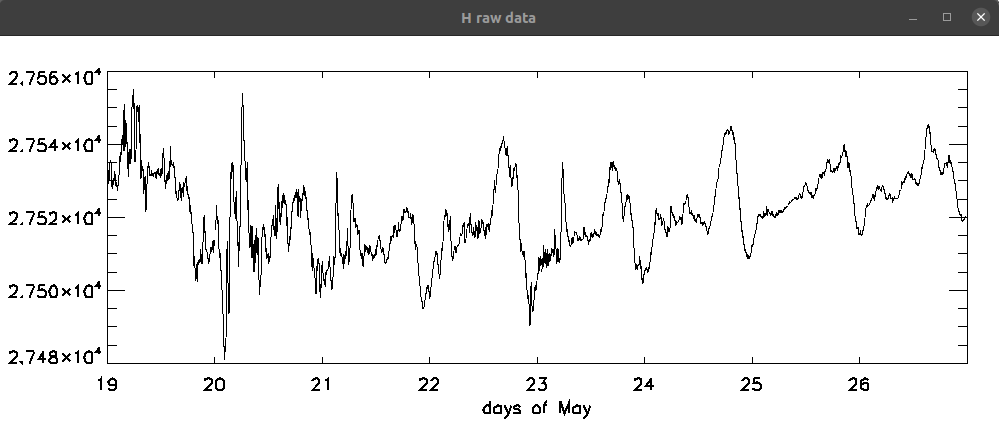
\includegraphics[width=10.0cm]{Images/cap2/lineabase/diadia/paso1.1.png}
     \centerline{\Large \bf   
         \hfill}
     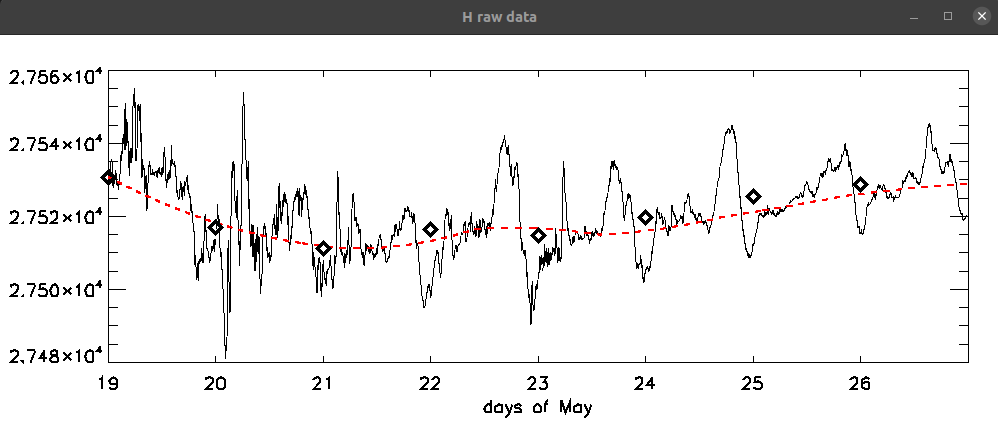
\includegraphics[width=10.0cm]{Images/cap2/lineabase/diadia/paso1.2.png}     
     \centerline{\Large \bf   
         \hfill}
      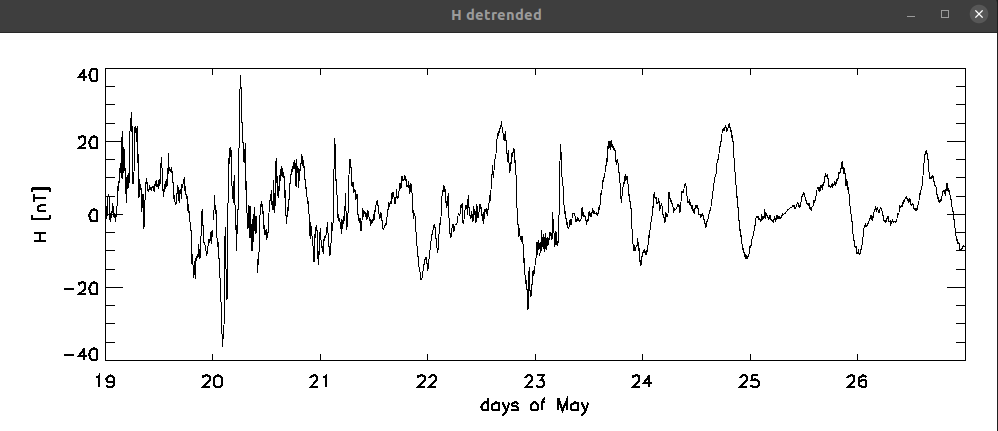
\includegraphics[width=10.0cm]{Images/cap2/lineabase/diadia/paso1.3.png}         
       \caption{Datos de salida de campo magnético, proporcionados por TEO(arriba), los rombos abiertos señalan los valores típicos (en medio) y su interpolación (linea roja) que será la linea base $H_0$. Los efectos removidos se muestran en el panel inferior.}
    \label{fig:diadia1}
\end{figure*}

No obstante, existe un problema al momento de llevar a cabo este procedimiento en ventanas de tiempo que enmarquen una TG. El punto clave en este caso, es que los días de tormenta, como su nombre lo indica, no manejan valores típicos, sino que son valores de perturbados a extremos. Estos valores no típicos, terminan influyendo en la serie de tiempo calculada, deformándola tal y como se observa en el panel inferior de la Figura \ref{fig:diadia2}, específicamente los días 28 y 29 de mayo que corresponden a días de tormenta. 
\vspace{1 em}

\begin{figure*}[h!]
    \centering
    \centerline{\Large \bf   
      %\hspace{0.18\textwidth}  \color{black}{\Large{Res}}
       %\hspace{0.28\textwidth}  \color{black}{\Large{Res+TC}}
         \hfill}
          \centerline{\Large \bf   
         \hfill}
     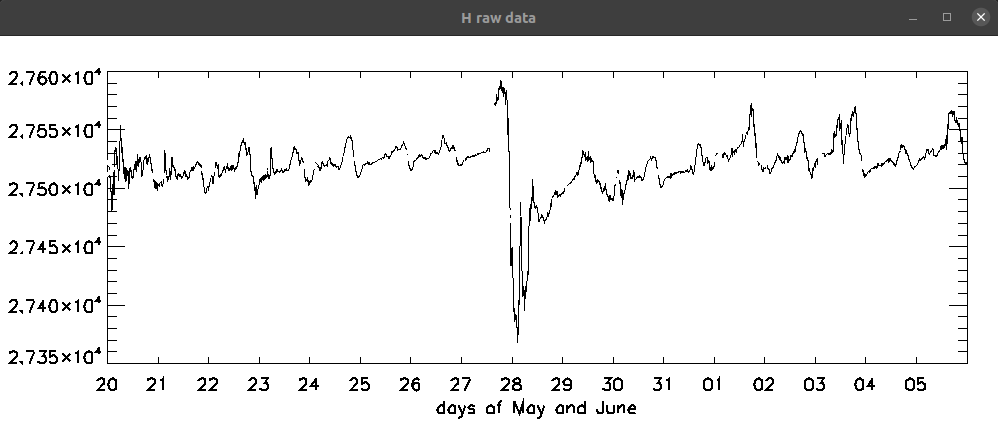
\includegraphics[width=10.0cm]{Images/cap2/lineabase/diadia/paso2.1.png}
     \centerline{\Large \bf   
         \hfill}
     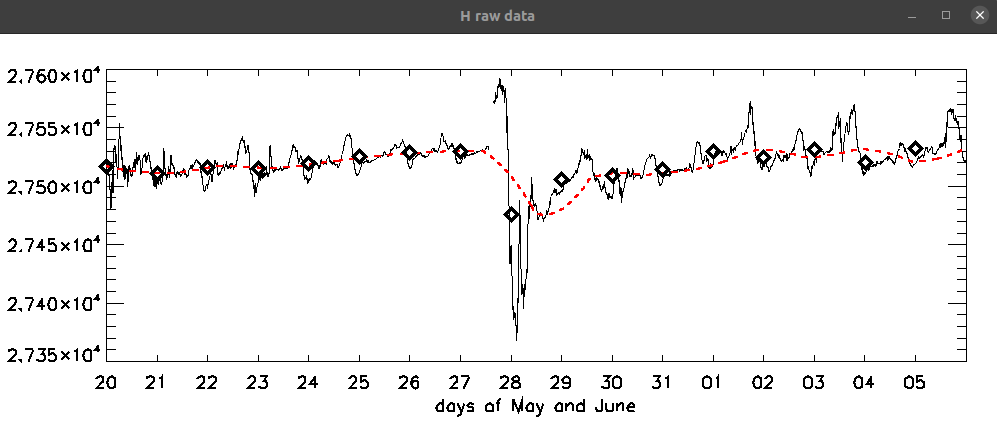
\includegraphics[width=10.0cm]{Images/cap2/lineabase/diadia/paso2.2.png}     
     \centerline{\Large \bf   
         \hfill}
      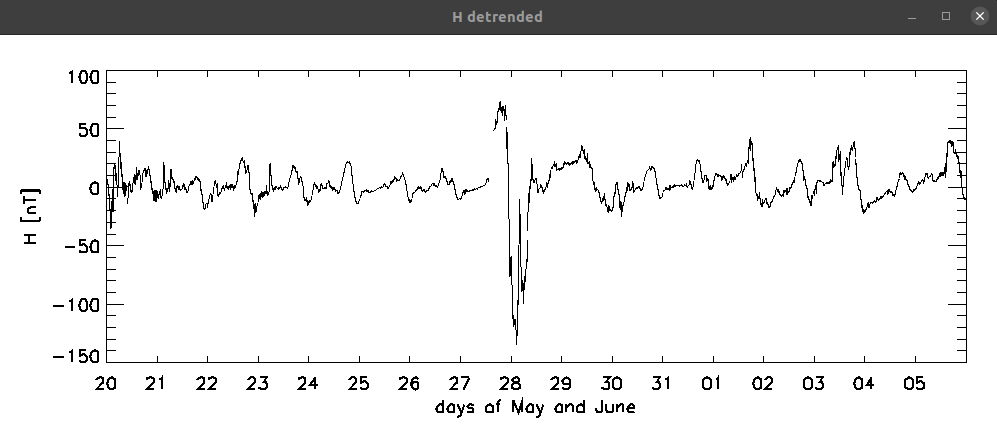
\includegraphics[width=10.0cm]{Images/cap2/lineabase/diadia/paso2.3.png}         
       \caption{Datos de salida de campo magnético para un evento de tormenta, proporcionados por TEO(arriba), los rombos abiertos señalan los valores típicos (en medio) y su interpolación (linea roja segmentada) que será la linea base $H_0$. Los efectos removidos se muestran en el panel inferior.}
    \label{fig:diadia2}
\end{figure*}

Para poder solucionar este problema, Es necesario considerar un umbral con el cual, el algoritmo de pre-procesamiento utilizado detecte los valores diarios asociados a periodos de tormenta. Así, todo valor que sobrepase el umbral será considerado como un día perturbado:
\begin{equation}
    \begin{split}
        LIM_{sup} = \Bar{H} + n \cdot \sigma \\
        LIM_{inf} = \Bar{H} - n \cdot \sigma,
    \end{split}    
\end{equation}
donde \emph{n} es un cualquier factor que se ajuste al caso de estudio (n=1.5 suele ser un buen valor para comenzar \cite{Dealing_with_outliers}) y $\Bar{H}$ es el promedio de la serie de tiempo que, en este caso, se trata de la componente horizontal del CMT local. \cite{baseline_Gjerloev, vanKampt} utilizan este criterio para los valores diarios de resolución 24h. Todo valor que se encuentre por fuera de este rango será considerado como valor nulo (NaN) y reemplazado usando una interpolación con los valores vecinos. En este trabajo, se consideró usar el criterio utilizado por \cite{phdthesis_ramon}, donde en vez de utilizar el promedio y la desviación estándar, se utilizan los cuartiles:

\begin{figure*}[h!]
    \centering
    \centerline{\Large \bf   
      %\hspace{0.18\textwidth}  \color{black}{\Large{Res}}
       %\hspace{0.28\textwidth}  \color{black}{\Large{Res+TC}}
         \hfill}
          \centerline{\Large \bf   
         \hfill}
     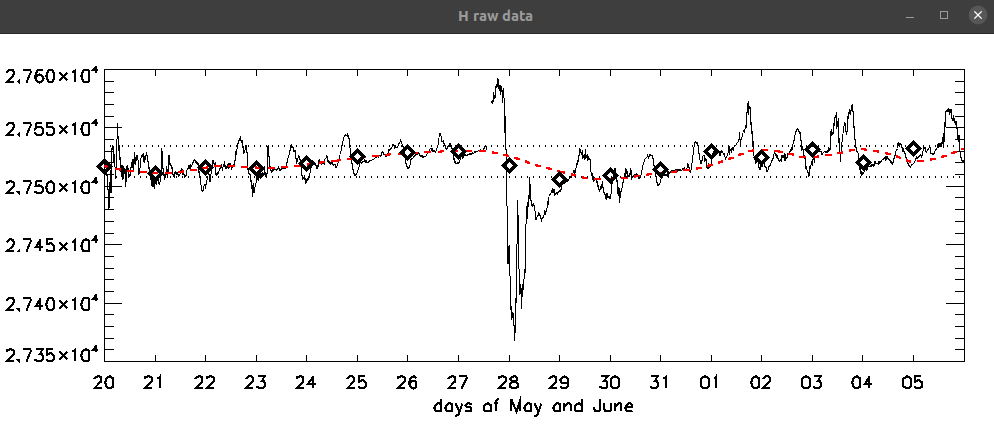
\includegraphics[width=10.0cm]{Images/cap2/lineabase/diadia/paso3.1.png}
     \centerline{\Large \bf   
         \hfill}
     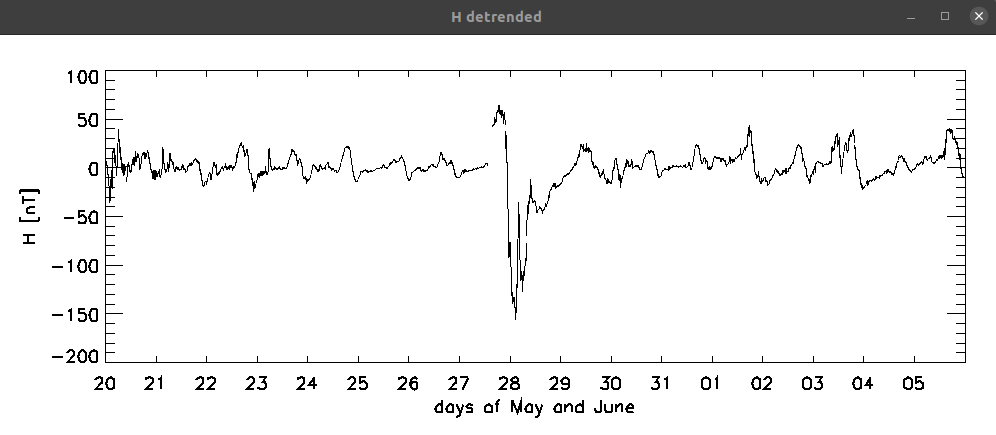
\includegraphics[width=10.0cm]{Images/cap2/lineabase/diadia/paso3.2.png}            
       \caption{Derivación corregida de la linea base $H_0$.}
    \label{fig:diadia3}
\end{figure*}


\begin{equation}
\label{eq:iqr}
    \begin{split}
        LIM_{sup} = M_{H} + n \cdot IQR \\
        LIM_{inf} = M_{H} - n \cdot IQR,
    \end{split}    
\end{equation}

La ventaja de utilizar el rango intercuartil así como la Mediana, se basa en que se tratan de valores estadísticos más robustos y menos sensibles al efecto de valores extremos que pudieran presentarse en la serie de tiempo. Gracias a este procedimiento, se podrá derivar de forma más precisa la linea base $H_0$ para periodos de tormenta. El resultado de este procedimiento se muestra en la Figura \ref{fig:diadia3}, donde ya no se observa la deformación de la serie de tiempo original, tal y como ocurre en la Figura \ref{fig:diadia2}. Cabe señalar que, de acuerdo con \cite{baseline_Gjerloev}, la cantidad de días que abarque la ventana de tiempo debe ser suficientemente grande, debido a que se derivará un dato por día. Es por ello que, para que los valores diarios tengan una significancia estadística, la ventana de tiempo debería ser de por menos 10 a 15 días, especialmente al considerar que la ventana de tiempo involucra días perturbados, los cuales serán descartados por medio del algoritmo.
\vspace{1 em}

\subsubsection{Linea base diurna}

La clave para la derivación de la línea base diurna son los días quietos. Se trata de los días oficialmente caracterizados por tener menor actividad geomagnética relacionada con la actividad solar. Para cada mes, se generan listas que contienen los datos de los diez días más quietos, tomando como referencia al índice Kp \cite{BARTELS_kp}. Cada mes, los datos son procesados en orden y promediados diariamente; los días con menor orden son los seleccionados como más quietos. La forma tradicional de derivar la linea base diurna es a través de promediar los datos magnéticos durante los cinco días más quietos. La información de los días más quietos de cada mes se encuentra en el sitio oficial del Servicio Internacional de Índices Geomagnéticos (ISGI por sus siglas en inglés), el cual proporciona la información de los días quietos derivados a partir del criterio antes mencionado.
\vspace{1 em}

Posteriormente, se genera una linea base a partir de este promedio que se denominará como $H_{SQ}$, la cual será restada de la serie de tiempo original o:
\vspace{1 em}

\begin{equation}
\label{eq:lineabase}
    H- H_0-H_{SQ}
\end{equation}

Sin embargo, una sumatoria de índices K puede llevar a un resultado engañoso ya que \textit{hay meses en que los días realmente quietos no ocurren. En estos casos, incluso aquellos 5 días seleccionados como menos perturbados presentan un nivel de perturbación tal que, en meses verdaderamente quietos, sus valores serían considerados como relativamente perturbados} \cite{BARTELS_kp}.
\vspace{1 em}

Por otro lado, existe un segundo problema que está relacionado con el objetivo de este trabajo: así como las perturbaciones geomagnéticas varían dependiendo de la región de estudio, también hay variaciones en periodos de quietud geomagnética. Mientras que para una región, puede haber un periodo de quietud geomagnética, en otra región pueden presentarse variaciones significativas, por lo que tal día ya no se consideraría quieto. Así, días considerados como quietos según el índice Kp, podrían ser no del todo quietos a escala local. Es por ello, que para considerar los días más quietos, éstos deben seleccionarse con base en datos magnéticos locales (y no planetarios, como es el caso de los días proporcionados por el ISGI). 
\vspace{1 em}

El criterio utilizado en este trabajo es el mismo seguido por \cite{baseline_Gjerloev, vanKampt}, de la máxima fluctuación diaria. Para una ventana de tiempo con suficientes días y con una resolución de 1 minuto, se hace un re-muestreo de los datos a 1h. Cada hora, se calcula la desviación estándar (como en \cite{vanKampt}) o bien, como se hizo en este caso, utilizando el rango intercuartil. Éstos valores horarios describen el grado de variación magnética, siendo el siguiente paso, seleccionar la máxima variación por cada día o el $MAX(\sigma)/MAX(IQR)$. Aquellos picos diarios de menor valor en la ventana de tiempo, serán considerados como días quietos locales o \emph{DQL}.
\vspace{1 em}

El siguiente paso es el de generar la linea base, y para ello, \cite{vanKampt} considera que no es necesario utilizar los 5 días quietos por cada mes. El motivo es que habrían meses altamente perturbados, donde los días clasificados como quietos en realidad no sean del todo ``quietos'', por lo que un promedio de éstos podría no ser la mejor opción. Esto sin mencionar que solamente 1 o dos días podrían considerarse como verdaderamente quietos. En su lugar, \cite{vanKampt} utiliza únicamente dos \emph{DQL}: un día previo al evento y el segundo posterior al evento, enmarcando a la TG. Entre más cercanos (temporalmente) sean los DQL entre sí, la linea base será más precisa, aunque el umbral de separación entre los \emph{DQL} puede ser de hasta 66 días \cite{vanKampt}.
\vspace{1 em}

A partir de aquí, \cite{vanKampt} aplica un análisis de Fourier, generando la serie de tiempo $H_{SQ}$ a base de un filtro pasa-bajas, para solo considerar las fluctuaciones asociadas a la variación diurna. Para este trabajo inicialmente se combinó con el criterio de \cite{baseline_Gjerloev} realizando una interpolaron linealmente los DQL al medio día sin aplicar previamente el filtro basa-bajas. A esta interpolación se le aplicó una función de suavizado por cada 30 minutos, siendo la serie resultante, la linea base $H_{SQ}$. En la Figura \ref{fig:diasq} se puede observar el procedimiento llevado a cabo. En el panel superior se muestra que a partir de dos DQL se generan dos series de tiempo (lineas azul y roja), haciendo la interpolación se genera la linea base $H_{SQ}$ a la cual se le aplica la función de suavizado. Posteriormente, en el panel inferior se muestra el resultado de remover este efecto descrito en la Ecuación \ref{eq:lineabase}. La linea negra representa la serie de tiempo previa a remover el efecto $H_{SQ}$, mientras que la linea roja representa la serie de tiempo, removiendo $H_{SQ}$. Se puede apreciar una atenuación de los efectos de variación diurna para cada día, sin que éste afecte a los valores durante el periodo en que ocurre la TG.
\vspace{1 em}


\begin{figure*}[h!]
    \centering
    \centerline{\Large \bf   
      %\hspace{0.18\textwidth}  \color{black}{\Large{Res}}
       %\hspace{0.28\textwidth}  \color{black}{\Large{Res+TC}}
         \hfill}
          \centerline{\Large \bf   
         \hfill}
     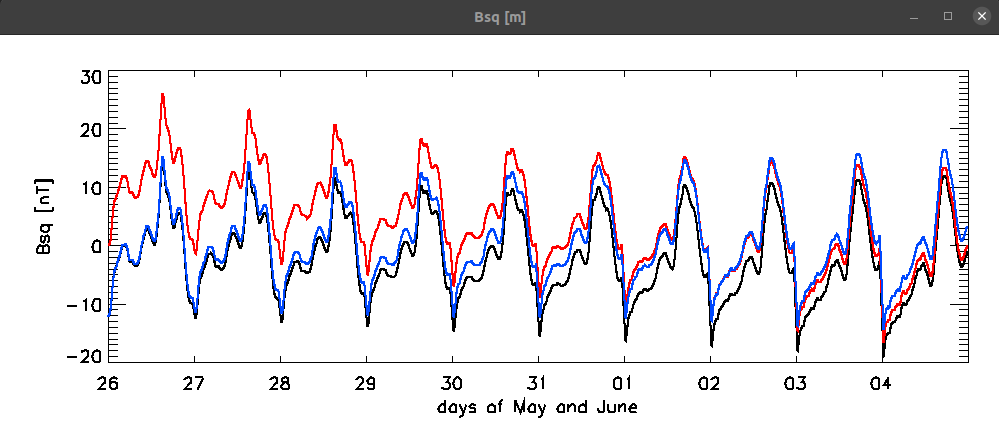
\includegraphics[width=10.0cm]{Images/cap2/lineabase/diurno/sq.png}
     \centerline{\Large \bf   
         \hfill}
     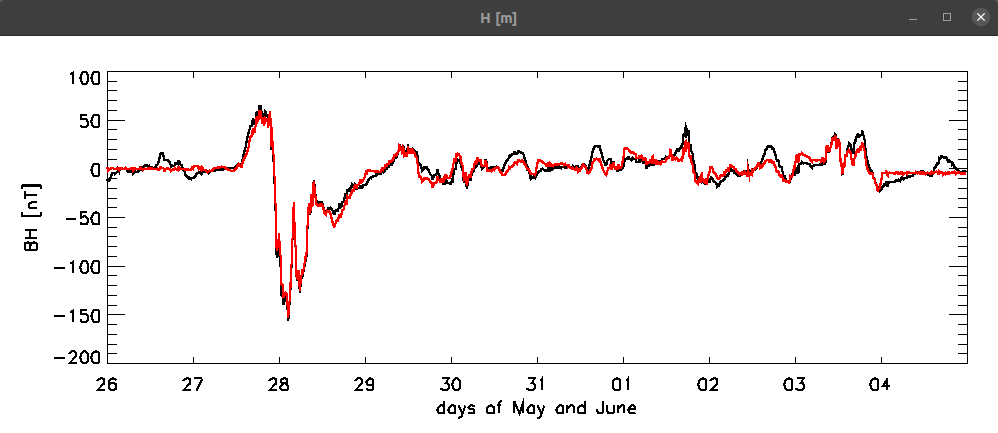
\includegraphics[width=10.0cm]{Images/cap2/lineabase/diurno/sq2.png}            
       \caption{Derivación de la linea base $H_{SQ}$.}
    \label{fig:diasq}
\end{figure*}


\subsection{valores extremos: picos de datos}
Una de las dificultades que se presentan al pre-procesar los datos de campo magnético son los valores extremos. Éstos valores pueden afectar los análisis posteriores, por lo que es sumamente importante poder generar un algoritmo que los detecte y elimine de la serie de tiempo a pre-procesar.
\vspace{1 em}

Los valores extremos en los datos son valores que se desvían de la tendencia general en las observaciones, tal y como se observa en el panel superior de la Figura \ref{fig:picos}. En general, pueden indicar una variabilidad en mediciones experimentales o tratarse de errores en las mediciones\cite{brief_overview_outlier-detection}.
\vspace{1 em}

Dependiendo del tipo de medición, los valores extremos pueden ser del tipo: puntuales, contextuales o colectivos. 

\begin{enumerate}
    \item Los valores puntuales o picos, son valores únicos cuya magnitud se aleja del resto de los datos en la distribución.
    \item Los contextuales se refieren al ruido de fondo en los datos.
    \item Los colectivos pueden tratarse de subconjuntos de novedades en los datos, como una señal que podría tratarse de un caso de interés.
\end{enumerate}

Las causas principales de estos valores extremos son:
\begin{itemize}
    \item errores en los datos de entrada (errores del operador)
    \item errores de medición (error instrumental)
    \item errores experimentales (datos de extracción o planteamiento experimental/ejecución de errores)
    \item intencional (errores aleatorios para prueba)
    \item errores de procesamiento de datos (manipulación de datos)
    \item errores de muestreo
    \item naturales (no necesariamente un error, sino un fenómeno no contemplado)
\end{itemize}

El detectar valores extremos como los picos, es de gran importancia en casi cualquier disciplina, por lo que es necesario considerar las siguientes interrogantes: ¿Cuales y cuantas características se considerarán para detectarlos?¿Se puede asumir las distribuciones de los valores para las características seleccionadas?
\vspace{1 em}

Algunos de los métodos más populares para la detección de valores extremos son:

\begin{itemize}
    \item Registro Z
    \item modelado de probabilidad y estadística
    \item modelos de regresión lineal
    \item modelos basados en proximidad
    \item modelos de información teórica
\end{itemize}

\subsubsection{Algoritmo de Whitaker-Hayes}
Se trata de un método altamente eficiente para lidiar con la detección de valores extremos únicos o picos \cite{Dealing_with_outliers}. Una ventaja que proporciona este algoritmo es que es lo suficientemente poco costoso, computacional mente hablando, como para ser ejecutado por la mayoría de sistemas computacionales \cite{WHITAKER2018}. Es necesario considerar sin embargo, que los datos deben tener una distribución cercana a la normal \cite{Dealing_with_outliers, brief_overview_outlier-detection}.
\vspace{1 em}

Éste algoritmo hace uso de una versión modificada del \emph{Puntaje Z}. Este método es un buen inicio para el tratamiento de valores extremos \cite{removing_with_Whitaker-Hayes}. Consiste en determinar qué tan alejado está un determinado valor con respecto a un promedio o mediana en la distribución de datos, usando medidas de variaciones (desviación estándar o rango intercuartil). El \emph{Puntaje Z} se calcula a partir de una serie de tiempo H de la siguiente forma:

\begin{equation}
    |z(i)| = | \frac{(H(i)-\Bar{H})}{\sigma} |
\end{equation}
Para detectar picos usando el \emph{Puntaje Z} es necesario ajustar los umbrales superiores e inferiores \cite{Dealing_with_outliers, removing_with_Whitaker-Hayes}.
\vspace{1 em}

Como mejor alternativa, uno puede hacer uso del \emph{Puntaje Z modificado} o \emph{PZM}. Éste método utiliza la desviación de la mediana absoluta (DMA), en lugar del promedio y se calcula de la siguiente forma:
\begin{equation}
    |z(i)| = | 0.6745 \cdot \frac{H(i) - M}{DMA}|,
\end{equation}
donde $DMA = |H-M|$, siendo $M$ la mediana de la serie de tiempo H(i). La ventaja es que la mediana y DMA son medidas más robustas de la tendencia central y la dispersión respectivamente. El multiplicador de 0.6745 es el cuartil 75 de la distribución normal estándar \cite{removing_with_Whitaker-Hayes}.

Para poder lidiar con los picos \cite{WHITAKER2018, removing_with_Whitaker-Hayes} consideran sus características de tener una alta diferencia con respecto de sus valores vecinos, así como un efecto de aumento agudo (no gradual). De esta forma, consideran que usando una derivada de primer orden en los datos consecutivos o $\nabla H(i) = H(i)- H(i-1)$ para calcular el PZM. Se observará un efecto de aplanamiento sobre las variaciones graduales, mientras que los picos que son delgados y de incremento agudo, son preservados, tal y como se aprecia en el panel de en medio de la Figura \ref{fig:picos}. Así, el algoritmo se expresa de la siguiente forma:
\begin{equation}
    |z(i)| = | 0.6745 \cdot \frac{\nabla H(i) - M}{MDA}|
\end{equation}

el criterio propuesto por la \emph{Sociedad Americana de Control de Calidad} es a partir de 3.5 , aunque de acuerdo con \cite{removing_with_Whitaker-Hayes}, el umbral dependerá de la serie de tiempo. El paso final es reemplazar por valores nulos y, en caso de ser necesario, es posible reemplazarlos a partir de una interpolación con los valores vecinos, tal y como se muestra en la Figura \ref{fig:picos}.

\begin{figure*}[h!]
    \centering
    \centerline{\Large \bf   
      %\hspace{0.18\textwidth}  \color{black}{\Large{Res}}
       %\hspace{0.28\textwidth}  \color{black}{\Large{Res+TC}}
         \hfill}
          \centerline{\Large \bf   
         \hfill}
     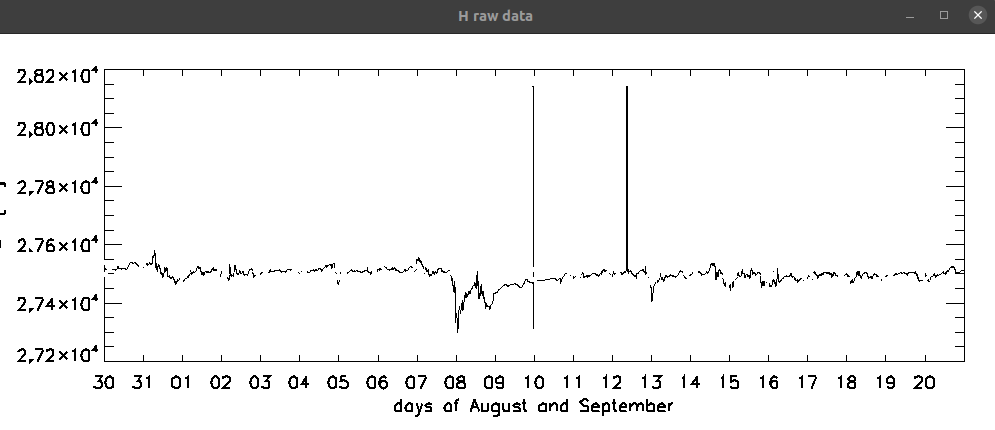
\includegraphics[width=10.0cm]{Images/cap2/lineabase/picos/picos.png}
     \centerline{\Large \bf   
         \hfill}
     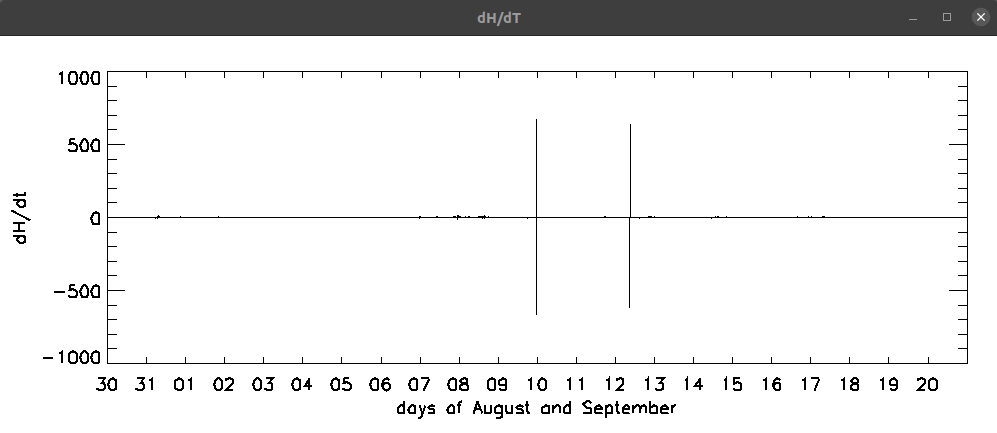
\includegraphics[width=10.0cm]{Images/cap2/lineabase/picos/picos2.png}     
     \centerline{\Large \bf   
         \hfill}
      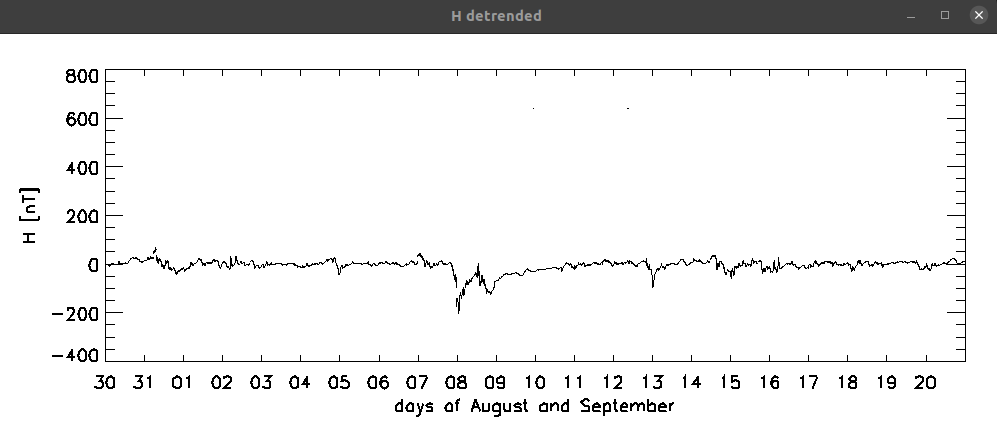
\includegraphics[width=10.0cm]{Images/cap2/lineabase/picos/picos3.png}         
       \caption{Datos de salida de campo magnético para un evento de tormenta, proporcionados por TEO(arriba), los rombos abiertos señalan los valores típicos (en medio) y su interpolación (linea roja) que será la linea base $H_0$. Los efectos removidos se muestran en el panel inferior.}
    \label{fig:picos}
\end{figure*}

\section{Análisis de Señales}

\subsection{Teorema de Percival y el Espectro de potencia}
\label{psd_section}
De acuerdo con el teorema de Percival, la energía de la señal se relaciona con la contribución de la densidad de energía en el sistema, a partir del parámetro a medir \cite{book_analysis_Method_multiSp_data}. La relación de Percival se describe por medio de la siguiente expresión: 

\begin{equation}
    \frac{1}{T} \int_{t0}^{t0+T} H^2(t)dt = \Tilde{H}[0] + 2 \sum_{n=1}^\infty |\Tilde{H}[n]^2|
\end{equation}

Los términos de la ecuación dependen de la longitud del intervalo T. Mientras que el lado izquierdo de la ecuación permanece igual (al modificar T), el lado derecho tendrá un cambio en el espaciamiento de las frecuencias $\Delta f = 1/T$. Entonces, los coeficientes en $|\Tilde{H}[n]|$ dependen de la longitud de la señal. Para poder describir entonces la distribución de la densidad de la energía de la señal en el espacio de frecuencias, introducimos la función \emph{PSD}:

\begin{equation}
    PSD[n] = 2T |\Tilde{H}|^2
\end{equation}

para todo $n$ positivo. Entonces, la relación de Percival toma la forma de:

\begin{equation}
    \frac{1}{T} \int_0^T H^2 (t)dt = PSD[0] \frac{\Delta f}{2} +2 \sum_{n=1}^\infty PSD[n] \Delta f
\end{equation}

Habiendo definido \emph{PSD}, su valor para una frecuencia en particular no cambiará con distintos T. La \emph{PSD} tiene una interpretación física inmediata: se trata de la contribución de la energía de la señal a partir de cada intervalo de frecuencia $\Delta f$ alrededor de $f_n$. Esto solo puede ser usado para frecuencias reales, ya que ignora las del conjunto imaginario.
\vspace{1 em}

La otra parte de la señal se encuentra en el espectro de fase, definido como:
\begin{equation}
    \Tilde{H}[n] = |\Tilde{H}[n]| exp(i\varphi [n]), 
\end{equation}

donde $\varphi [-n] = -\varphi[m]$ y $\varphi[0]=0$. el valor absoluto de la fase depende de la posición inicial del muestreo de la señal.
\vspace{1 em}

\subsubsection{Función Ventana}

Considerando que, tanto la transformada discreta de Fourier como PSD consideran las series de tiempo como infinitas, al usar series de tiempo de duración finita conduce a un problema: el efecto de borde. La abrupta interrupción en una ventana de tiempo usada (denominada como rectangular) ocasiona una pérdida de energía desde cualquiera de los picos espectrales, hacia las frecuencias vecinas. Esto se debe a que el efecto escalón debido al borde provoca una dispersión en la energía, la cual es transferida \cite{book_analysis_Method_multiSp_data}.
\vspace{1 em}

Como solución para este fenómeno, se han diseñado una gran variedad de funciones ventana. Se trata de un subconjunto de la serie de tiempo (o sub-ventanas de la ventana original) a la cual se le aplica una función, la cual se irá recorriendo para toda la serie de tiempo. Como tal, las funciones ventanas no pueden llevar la pérdida de frecuencia a cero, sin embargo tienen la capacidad de atenuar la pérdida de energía que normalmente se dispersa hacia las demás frecuencias, ocasionando un incremento en el grosor del pico principal.
\vspace{1 em}

En este punto, es importante dedicar esfuerzo a la selección de parámetros de la ventana (y a la selección de la función ventana). No obstante, el objetivo principal es \textbf{no usar una ventana rectangular}.
\vspace{1 em}

En general, al multiplicar la señal por coeficientes de las ventanas (que suelen ser menores a 1), se obtiene una pérdida general de la energía. Esta pérdida depende de la señal en sí, pero al considerar la relación de Percival, se tiene que el decremento estadístico esperado de los valores del PSD debido a la función ventana es del promedio del cuadrado de la ventana:

\begin{equation}
    W_{pc} = \frac{1}{N} \sum_{j=0}^{N-1} w[j]^2,
\end{equation}

por lo que para compensar la pérdida de energía en el PSD, posterior a la aplicación de la función ventana, el PSD debe dividirse por $W_{pc}$.
\vspace{1 em}

\subsection{Análisis de Ondículas}

La técnica para representar variaciones rápidas en el dominio de la frecuencia y variaciones lentas en el dominio del tiempo se conoce como análisis tiempo-frecuencia. La relación entre tiempo-frecuencia (alta-baja resolución) depende de las propiedades de la señal, para saber si se quiere que el tiempo tenga mayor resolución, a expensas de resolución en frecuencia o viceversa \cite{book_analysis_Method_multiSp_data}. La aplicación de este tipo de análisis tiene ciertas ventajas, ya que permite detectar el momento en el tiempo en que se presentan ciertas fluctuaciones a determinada frecuencia. Esto es algo que no puede observarse en los espectros de potencia, donde sólo se muestran los picos de potencia, pero no se muestra el tiempo en que se presentan (bien puede tratarse de un efecto limitado a un corto periodo, o un efecto persistente). Esta es la idea del uso de las ondículas, pues el poder localizar en tiempo determinadas fluctuaciones a ciertas frecuencias o trenes de ondas implica una ventaja al no saber si se trata de una señal persistente o muy breve en la ventana. 
\vspace{1 em}

La transformada Wavelet o de ondícula puede ser utilizada para analizar series de tiempo que contengan una potencia no estacionaria en diferentes frecuencias \cite{guide_wavelet_routines}. De la misma forma, es necesario considerar la forma o función de la ondícula $\psi_0(n)$ donde $n$ es un parámetro de tiempo. Una función ondícula, como la ondícula Morlet tiene la siguiente forma:

\begin{equation}
    \psi_0(n) = \pi^{1/4}e^{i \omega_0 n} e ^{-n^2/2}
\end{equation}

donde $\omega_0$ es una frecuencia adimensional. El término función wavelet o de ondícula se refiere a ondículas ortogonales o no ortogonales. Para series de tiempo discretas, se utiliza una transformada discreta que tiene la siguiente forma: 

\begin{equation}
    W_n(s) = \sum_{k = 0}^{N-1} \hat{x}_k \hat{\psi} \ast (s \omega_k) e^{i \omega_k n {\displaystyle \delta} t}
\end{equation}

donde $\hat{x}_n$ es una transformada discreta de Fourier, $k=0...N-1$ es el índice de las frecuencias, $s$ es la escala que permite modificar la amplitud de la forma sinusoidal resultante y la frecuencia angulas $\omega_k$ se define como:

\begin{equation}
    \begin{split}
        \omega_k = \frac{2 \pi k}{N {\displaystyle \delta} t} : k \le \frac{N}{2}\\
        \omega_k = - \frac{2 \pi k}{N {\displaystyle \delta} t} : k > \frac{N}{2}
    \end{split}
\end{equation}

Una practica común \cite{book_analysis_Method_multiSp_data, guide_wavelet_routines} es la de normalizar las transformadas de ondícula, para que puedan compararse unas con otras, mediante la siguiente expresión:

\begin{equation}
    \hat{\psi}(s \omega_k) = (\frac{2 \pi s}{{\displaystyle \delta} t} )^{1/2} \hat{\psi}_0 (s \omega_k)
\end{equation}

Por otro lado, así como es posible obtener la energía de la señal derivada a partir del teorema de Percival, también es posible hacer lo propio con la transformada de ondícula, siendo ésta la potencia espectral de la ondícula definida como $|W_n(s)|^2$. Al igual que con los \emph{PSD}, la potencia de la ondícula permite visualizar los picos de energía de las frecuencias más significativas, con la diferencia en que también se obtiene información en el dominio del tiempo.
